\documentclass[mathserif, aspectratio=169]{beamer}
\usetheme{odenpecos}
\setbeamertemplate{itemize/enumerate body begin}{\fontsize{8.8}{9}\selectfont}
\setbeamertemplate{itemize/enumerate subbody begin}{\fontsize{7.5}{8}\selectfont}
\setbeamertemplate{itemize/enumerate subsubbody begin}{\fontsize{7.5}{8}\selectfont}

% default search path for figures
\graphicspath{{../fig/}}

\newcommand{\zapspace}{\topsep=0pt\partopsep=0pt\itemsep=0pt\parskip=0pt}

\usepackage{multicol}
\usepackage{multirow}
\usepackage{pict2e}
%\usepackage{esdiff}
\usepackage{multimedia}
\usepackage{verbatim}
\usepackage{mhchem}
\usepackage{tikz}
\usetikzlibrary{arrows}
\usepackage[percent]{overpic}
\usepackage[absolute,overlay]{textpos}
\usepackage{tikz} % Required for flow chart
\usepackage[caption=false]{subfig}

\newcommand{\overbar}[1]{\mkern 1.5mu\overline{\mkern-1.5mu#1\mkern-1.5mu}\mkern 1.5mu}
\newcommand{\pp}[2]{\frac{\partial #1}{\partial #2}}
\newcommand{\dd}[2]{\frac{d #1}{d #2}}
\newcommand{\DD}[2]{\frac{D #1}{D #2}}
\newcommand{\mm}{\mathbf{minmod}}
\def\etal{{\it et al~}}
\newcommand{\be}{\begin{eqnarray}}
	\newcommand{\ee}{\end{eqnarray}}
\newcommand{\mbb}[1]{\mathbb{#1}} % math blackboard bold
\newcommand{\mcal}[1]{\mathcal{#1}} % math blackboard bold
\newcommand{\mbf}[1]{\mathbf{#1}} % math bold face (for vectors)
\newcommand{\sbf}[1]{\boldsymbol{#1}} % bold face for symbols
\newcommand{\jump}[1]{\llbracket #1 \rrbracket} % jump operator
\newcommand{\avg}[1]{\langle #1 \rangle} % average operator
\newcommand{\rarrow}{\rightarrow}
\newcommand{\Rarrow}{\Rightarrow}
\newcommand{\LRarrow}{\Leftrightarrow}
\newcommand{\vvvert}{|\kern-1pt|\kern-1pt|}
\newcommand{\enorm}[1]{\vvvert #1 \vvvert}
\newcommand{\nutil}{\tilde{\nu}}
\newcommand{\Var}{\mathrm{Var}}
\newcommand{\Cov}{\mathrm{Cov}}


\definecolor{MyDarkGreen}{rgb}{0,0.45,0.08}
\newcommand{\myred}[1]{{\color{red} #1}}
\newcommand{\myblue}[1]{{\color{blue} #1}}
\newcommand{\mygreen}[1]{{\color{MyDarkGreen} #1}}

\newcommand{\sa}{\nu_{\mathrm{sa}}}
\newcommand{\tep}{\tilde{\epsilon}}
\newcommand{\Ssd}{\mathcal{S}} % source term due to slow derivative
\newcommand{\ud}{\,\mathrm{d}}

\newcommand{\Mach}[1]{\ensuremath{\mbox{Ma}_{#1}}}
\newcommand{\Reynolds}{\ensuremath{\mathit{Re}}}
\newcommand{\DensityRat}{\ensuremath{\mathit{DR}}}
\newcommand{\BlowRat}{\ensuremath{\mbox{BR}}}
\newcommand{\VelRat}{\ensuremath{\mathit{VR}}}
\newcommand{\Tau}{\ensuremath{\mathrm{T}}}

\newcommand{\wall}     {\ensuremath{\mathrm{w}}}   % wall subindex
\newcommand{\awall}    {\ensuremath{\mathrm{aw}}}  % adiabatic wall subindex

\newcommand{\commentout}[1]{}

\newcommand{\vect}[1]{\boldsymbol{#1}}
\usepackage{mleftright}
\newcommand{\of}[1]{\mleft( #1 \mright)}
\newcommand{\vth}{v_{\textrm{th}}}
\newcommand{\reals}{\mathbb{R}}
\newcommand{\myint}{\int\limits}
\newcommand{\ddt}[1]{\partial_t #1}
\newcommand{\RR}{\mathbb{R}}
\newcommand{\vr}{v}
\newcommand{\diff}[1]{\, d#1}
\newcommand{\norm}[1]{\left\lVert#1\right\rVert}
%\newcommand{\vtheta}{\theta_{\vect{v}}}
%\newcommand{\vphi}{\varphi_{\vect{v}}}
%\newcommand{\vr}{v_{r}}
\newcommand{\vtheta}{{v_{\theta}}}
\newcommand{\vphi}{v_{\varphi}}
\newcommand{\vomega}{v_{\omega}}
\newcommand{\vrunit}{\hat{\vect{v}}_{r}}
\newcommand{\vthetaunit}{\hat{\vect{v}}_{\theta}}
\newcommand{\vphiunit}{\hat{\vect{v}}_{\varphi}}
\DeclareMathOperator{\variance}{Var}

\usepackage{mathtools}
\DeclarePairedDelimiter\ceil{\lceil}{\rceil}
\DeclarePairedDelimiter\floor{\lfloor}{\rfloor}

\begin{document}
% disable nav
\setbeamertemplate{navigation symbols}{}

% ---------------------------------------------------------------
% Oden/Pecos title page

\hoffset=.16in

\begin{frame}[plain,t]{}
\makeatletter
%\vspace*{0.85cm}
%\vspace*{0.65cm}
\includegraphics[height=0.9in,trim=50 40 40 0, clip]{PMSc_159_university_formal_horizontal.pdf} \newline
%\vspace*{0.3cm}
\begin{columns}[T,onlytextwidth]
\column{.8\textwidth}
{\bf \color{burntorange} \fontfamily{bch}\selectfont 
% -- Set talk title here
Solving the Boltzmann equation for electron kinetics using Galerkin approach
% --
}
\end{columns}
\vspace*{.15cm}
\rule{.8\textwidth}{0.6pt} \newline

\vspace*{0.05cm}
\setstretch{0.65}
{\fontfamily{phv}\selectfont
  { \scriptsize
    % -- define presenter, authors here
    Milinda Fernando \\%, Todd Oliver, Laxminarayan Raja, Philip Varghese, Robert Moser, George Biros  \\
    % --
  }
  {\color{burntorange} \tiny
    % -- define role, meeting event, location, etc
    PSAAP III Annual Review $\cdot$ November 08-09, 2023
    %PSAAP TST Meeting $\cdot$ April 24-25, 2023
    % --
  }
}

\vspace*{1cm}
%\includegraphics[height=0.3in]{figures/pecos_orange1.png}
\begin{columns}
\begin{column}{0.8\linewidth}
\includegraphics[height=0.5in]{oden_pecos_2020_wordmark.png}\\
{\scriptsize \url{https://pecos.oden.utexas.edu}}
\end{column}

\begin{column}{0.2\linewidth}
\includegraphics[height=0.6in]{psaap3-logo.png}
\end{column}
\end{columns}

\end{frame}
\hoffset=0in
% -- end title slide ---------------------------------------------

%\begin{frame}
%	\frametitle{Outline}
%	\begin{itemize}
%		\item Spatially homogeneous Boltzmann equation, $\partial_t f - \frac{\vect{E} q}{m} \cdot \nabla_{\vect{v }}f = C(f)$
%		\item Representation of $f$ (i.e., isotropic + anisotropic correction terms), use spherical harmonics for angular directions + experimentation of basis functions in radial direction. 
%		\begin{itemize}
%			\item Global approximations with Maxwell and Laguerre polynomials.
%			\item Local approximations with linear and higher order B-splines
%		\end{itemize}
%		\item Collision operator (5d integral form)
%		\item Simplifications for the collision operator with analytical integration of angular directions (1d integral form). 
%		\item Equations for the steady-state solution (spatially homogeneous case) 
%		\item Two-term formulation vs. EEDF formulation with diffusion term. 
%		\item Verification with Bolsig+ code.  (Both approaches, importance of the diffusion term), PS 2.4
%		\item Formulation for 1D-space+3D-velocity space Boltzmann equations with some preliminary results for 1d glow discharge problem. 
%		\item Discuss on single GPU implementation with CuPy, Challenges in 1D+3V formulation (i.e., boundary conditions) and Future work, ES 2.6
%	\end{itemize}
%\end{frame}

\begin{frame}[fragile]
	\frametitle{Where do we fit ? }
	% \begin{tikzpicture}
	% 	\node[anchor=south west,inner sep=0] at (0,0) {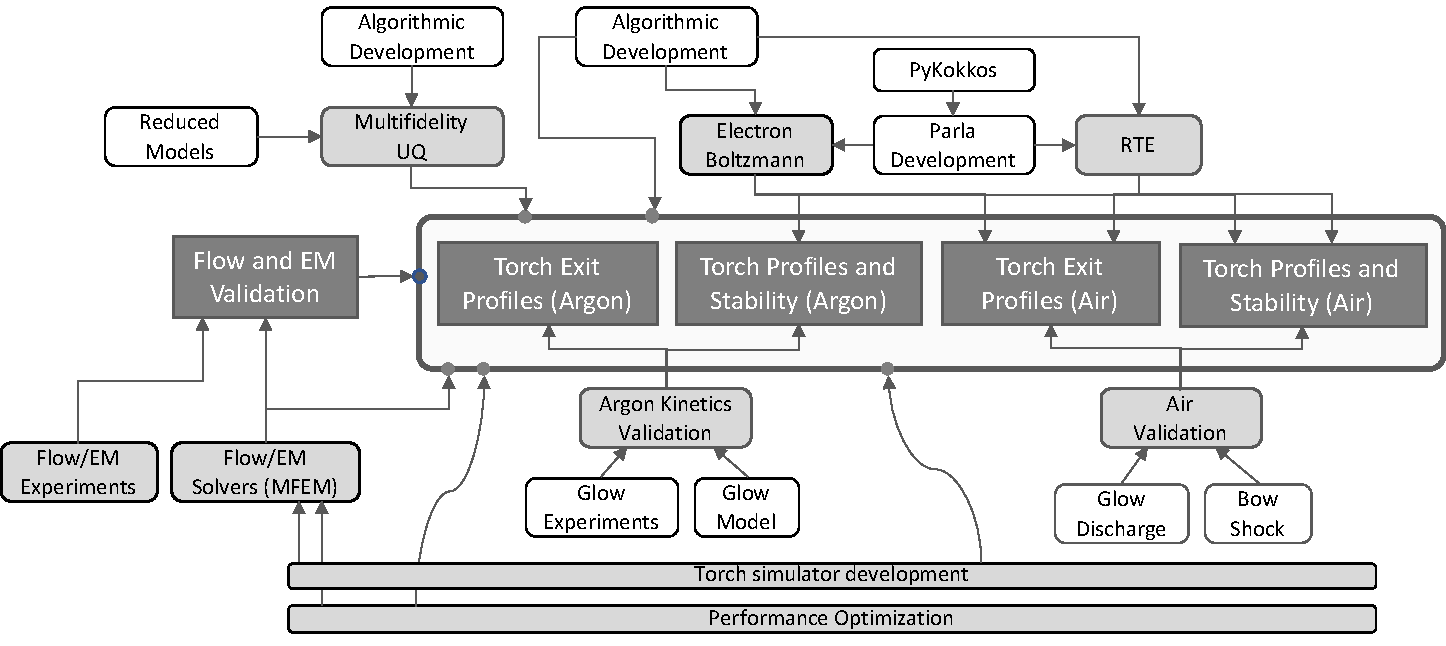
\includegraphics[width=0.8\textwidth]{pecos_roadmap_tst_1.5.pdf}};
	% 	\draw[orange, fill = yellow!30, fill opacity = 0.4 ,ultra thick,rounded corners] (4.15,3.6) rectangle +(4.2,1.6);
	% \end{tikzpicture}
	\begin{center}
		\includegraphics[width=0.9\textwidth]{where_we_fit.png}
	\end{center}
\end{frame}

\begin{frame}
	\frametitle{Outline}
	\begin{columns}
		\begin{column}{0.4\textwidth}
				\begin{itemize}
				\item Spatially homogeneous Boltzmann equation
				\item Formulation \& Discretization
				\item Collision operators
				\begin{itemize}
					\item electron-heavy collisions
					\item electron-electron collisions
				\end{itemize}
				\item Steady-state solutions
				\item Verification with Bolsig
			\end{itemize}
		\end{column}
		\begin{column}{0.6\textwidth}
			\begin{itemize}
				\item Year 1 : Discretization and formulation 
				\begin{itemize}
					\item B-Splines + Spherical harmonics (established)
				\end{itemize}	
				\item Year 2 : Verification with Bolsig
				\item Year 3 : Glow discharge problem
					\begin{itemize}
						\item Issues with the boundary condition
						\item Importance on the electron-electron collisions
					\end{itemize}
				\item \textbf{Completed}
				\begin{itemize}
					\item Verification with bolsig with electron-heavy and electron-electron collisions
					\item Beyond 2-term approximation
					\item Ability to handle cases without azimuthal symmetry
					\item Implementation of 1d2v glow-discharge with Boltzmann  
				\end{itemize}\textbf{}
			\end{itemize}
		\end{column}
	\end{columns}

%	\begin{itemize}
%		\item \large spatially homogeneous Boltzmann solver 
%		\begin{itemize}
%			\item Formulation
%			\item Discretization
%			\item Collision operators
%			\item Results
%			\item Verification with Bolsig+
%		\end{itemize}
%		\item 1D3V - Glow discharge problem
%		\begin{itemize}
%			\item \large Formulation
%			\item Discretization
%			\item Boundary conditions
%		\end{itemize}
%		\item Future work
%	\end{itemize}
	% \begin{itemize}
	% 	\item Current work on deterministic Boltzmann solver for 0D3V and 1D3V
	% 	\begin{itemize}
	% 		\item 0D3V solver
	% 		\begin{itemize}
	% 			\item Studied efficient discretization in speed
	% 			\item Verified 0D3V code with Bolsig+ in different parameter regimes
	% 		\end{itemize}
	% 		\item 1D3V solver
	% 		\begin{itemize}
	% 			\item Implemented CPU/GPU Python implementation
	% 			\item Currently, resolving issues with boundary conditions
	% 		\end{itemize}
	% 	\end{itemize}
	% 	\item 0D3V formulation and results
	% 	\item 1D3V formulation and preliminary results
	% \end{itemize}
\end{frame}



\begin{frame}
	\frametitle{Boltzmann equation}
	\begin{itemize}
		\item For a given electric field $\vect{E}$
		\begin{align}
			\partial_t f -\frac{\vect{E} q}{m} \cdot \nabla_{\vect{v }}f = C_{en}f + C_{ee}(f)
		\end{align}
		\item $C_{en}$ : electron-heavy collisions (i.e., elastic, ionization)
		\begin{itemize}
			\item Use LXCAT cross-section data 
			\item Linear in $f$
		\end{itemize} 
		\item $C_{ee}$ : electron-electron Columbic collisions 
		\begin{itemize}
			\item Modeled using Fokker-Plank equation with analytical cross-section
			\item Nonlinear in $f$
		\end{itemize}
		%\item $C_{ei}$: electron-ion Columbic can be modeled similarly if needed
%		\item Derived the steady state equation
%		\begin{align}
%			\textcolor{black!70}{\partial_t \hat{f} = -(u^T C \hat{f}) \hat{f} + (C+E)\hat{f} \text{ where } \hat{f}(\vect{v},t) = \frac{f(v,t)}{\myint_{R^3} f(\vect{v},t) \diff{\vect{v}}}}\\
%			\textcolor{black!70}{\partial_t (\hat{f}) = 0 \ \ \  \Rightarrow} \ \ \  -(u^T C \hat{f}) \hat{f} + (C+E)\hat{f} =0  \text{ with } u^T \hat{f}-1=0
%		\end{align}
	\end{itemize}
\end{frame}

\begin{frame}
	\frametitle{Challenges}
	\begin{columns}
		\begin{column}{0.3\textwidth}
			\begin{itemize}
				\item Non-smooth cross sections $\Rightarrow$ non-smooth $f$ solutions
				\item Strong advection may cause stabilization issues
				\item To compute QoIs $\rightarrow$ need accurate tails of $f$ 
			\end{itemize}
		\end{column}
		\begin{column}{0.7\textwidth}
			\vspace*{-0.8in}
			\begin{center}
				\includegraphics[width=\columnwidth]{g0_g2_cs.png}
			\end{center}
		\end{column}
	\end{columns}
\end{frame}

\begin{frame}
	\frametitle{Discretization}
	\small
	\begin{itemize}
		\item Representation of $f\of{\vect{v},t} = \sum_{klm} f_{klm} \underbrace{\phi_k\of{v}}_{\text{B-Spline basis}} \underbrace{Y_{lm}\of{v_\theta, v_\phi}}_{\tiny\text{sph. harm.}}$ 
		\item Weak formulation
			$
			\displaystyle
			\quad
			\partial_t f - \frac{\vect{E} q}{m} \cdot \nabla_{\vect{v}}f = C(f)
			\quad $ \\
			$
			\displaystyle
			\quad
			\Rightarrow \quad
			\partial_t \myint_{R^3} f \phi\of{\vect{v}} \ud \vect{v} = 
			\myint_{R^3} \of{C_{en}f + C_{ee}(f)} \phi\of{\vect{v}} \ud \vect{v} + \myint_{R^3} \of{\frac{\vect{E} q}{m} \cdot \nabla_{\vect{v}} f} \phi(\vect{v}) \ud \vect{v}\text{ , } 
			\forall \phi(\vect{v})$
		\item Weak form of the collision operator (5d integral) \\
			$
			\displaystyle
			\quad 
			\myint_{R^3} C_{en} \phi\of{\vect{v}_e} \diff{\vect{v}_e} 
			=
			N \myint_{R^3} \myint_{S^2} 
			v\sigma(v,\vect{\omega})
			f_e\of{\vect{v}_e}
			\left(
			\psi\of{\vect{v}_e^\text{post}\of{\vect{v}_e, \vect{\omega}}} 
			- \psi\of{\vect{v}_e} 
			\right)
			\diff{\vect{v}_e} \diff{\vect{\omega}}
			$
		\item Isotropic scattering, azimuthal symmetry, and using spherical harmonics addition (1d integral)\\
		$
		\displaystyle
		\quad 
		C_{en}^{ql} 
		=
		N \myint_{0}^{\infty} 
		v^3\sigma(v)\delta_{ql}
		f_e^{l}\of{v}
		\left(
		\delta_{q0}\psi\of{v_e^\text{post}\of{v}} - \psi\of{v} 
		\right)
		\diff{v} 
		$ 
	\end{itemize}
\end{frame}

\begin{frame}
	\frametitle{Electron-electron collisions}
	\begin{itemize}
		\item We use Rosenbluth's (1957) Fokker-Plank derivation for electron-electron collisions. Let $H=\partial^2_{ab}$
		\begin{align}
			C_{ee}(f) &= \Gamma_a(-\nabla \cdot (f \nabla h ) + \frac{1}{2} H : \of{f H g}) \text{ where } \Delta h  = -8\pi f \text{ and } \Delta^2 g =-8\pi f	
		\end{align}
		\item Assuming azimuthal symmetry, we can compute Rosenbluth potentials, 
		\begin{align}
			& h_a\of{\vect{v}} = \sum_{l} A^{b}_l\of{v} Y_{l0}\of{\vtheta, \vphi}  \text{ and } g\of{\vect{v}} = \sum_{l} B^{b}_l\of{v} Y_{l0}\of{\vtheta, \vphi}\text{ where } \\
			& A^{b}_l\of{v} = \frac{8\pi}{(2l+1)}\of{\int_{0}^{v} dv^\prime \frac{{v^\prime}^{l+2}}{v^{l+1}} f^{b}_l\of{v^\prime} +  \int_{v}^{\infty} dv^\prime \frac{{v}^{l}}{{v^\prime}^{l-1}} f^{b}_l\of{v^\prime}}\\
			B^{b}_{l}\of{v} & = -\frac{4\pi}{(4l^2-1)} \of
			{
				\int_{0}^{v} \diff{v^\prime} f^{b}_l\of{v^\prime} \frac{{v^\prime}^{l+2}}{v^{l-1}} \of{1 - \of{\frac{l-1/2}{l+3/2}}\of{\frac{{v^\prime}^2 }{v^2}}} } + \nonumber\\
			&-\frac{4\pi U_{l0}}{(4l^2-1)} \of{
				\int_{v}^{\infty} \diff{v^\prime} f^{b}_l\of{v^\prime} \frac{{v}^{l}}{{v^\prime}^{l-3}} \of{1 - \of{\frac{l-1/2}{l+3/2}}\of{\frac{{v}^2 }{{v^\prime}^2}}}
			}
		\end{align}
	\end{itemize}
\end{frame}

\begin{frame}
	\frametitle{Electron-electron collisions}
	\begin{itemize}
		\item Weak form of the coulomb collisions
		\begin{align}
			\int_{R^3} C_{ee}(f) \psi(\vect{v})\diff{\vect{v}} = \Gamma_a \of{\int_{R^3} \nabla \psi\of{\vect{v}} \cdot (f \nabla h ) \diff{\vect{v}}  + \frac{1}{2} \int_{R^3} H\psi\of{\vect{v}} : \of{f H g} \diff{\vect{v}}} 
		\end{align}
		\item For given test function $\psi_{pq}$, we can pre-compute 6th order tensor ${C_{ee}}_{rs,kl}^{pq}$
		\begin{align}
			[C_{ee}]_{rs,kl}^{pq} = \int_{R^3} C_{ee}(\phi_{rs}, \phi_{kl}) \phi_{pq} \diff{\vect{v}} 
		\end{align}
		\item SymPy based symbolic framework for weak form derivation in spherical coordinates
		\begin{itemize}
			\item Ability to derive equation for arbitrary order of polar modes
			\item Integrate the angular coordinates analytically, identification of the non-zero modes (i.e., sparse tensor) 
			\item Radial integration performed exactly using gauss quadrature on B-Splines
		\end{itemize}
	\end{itemize}
\end{frame}

\begin{frame}
	\frametitle{Transient and steady-state solutions}
	\begin{itemize}
		\item Steady-state solution for a given $E/N$ field and ionization degree $n_e/N$ 
		\begin{align}
			\partial_t {\hat{f}} &=(C_{en}+E)\hat{f} + n_e C_{ee}\of{\hat{f}} - \mu(\hat{f}) \hat{f} \text{ where } \mu(\hat{f}) = \frac{\partial_t n_e}{n_e} = u^T C_{en}(\hat{f})\\
			&\text{ with constraint } u^T \hat{f} = 1 \nonumber 
		\end{align}
		\item Use Newton's method with line search
		\item Implicit time integration
%		\item For steady-state solution we solve $\partial_t {\hat{f}} = 0$, with $R(\hat{f}) = (C_{en}+E)\hat{f} + n_e C_{ee}\of{\hat{f}, \hat{f}} - \mu(\hat{f})$, we can write the Jacobian $\frac{d R}{d\hat{f}} = J(\hat{f}) = C_{en} + E + n_e \of{C_{ee}\of{\cdot,\hat{f}} + C_{ee}\of{\hat{f},\cdot}} -\mu(\hat{f})I$
		%\item $\hat{f}^{n+1} = \hat{f}^{n} - \alpha [J(\hat{f}^n)]^{-1}R(\hat{f}^n)$, where $\alpha \in(0,1]$ determined by line-search algorithm 
	\end{itemize}
\end{frame}

\begin{frame}
	\frametitle{Effect of Columbic collisions}
	$E/N$ = 1Td with elastic + ionization with varying $n_e/N$
	\vspace*{-0.1in}
	\begin{center}
		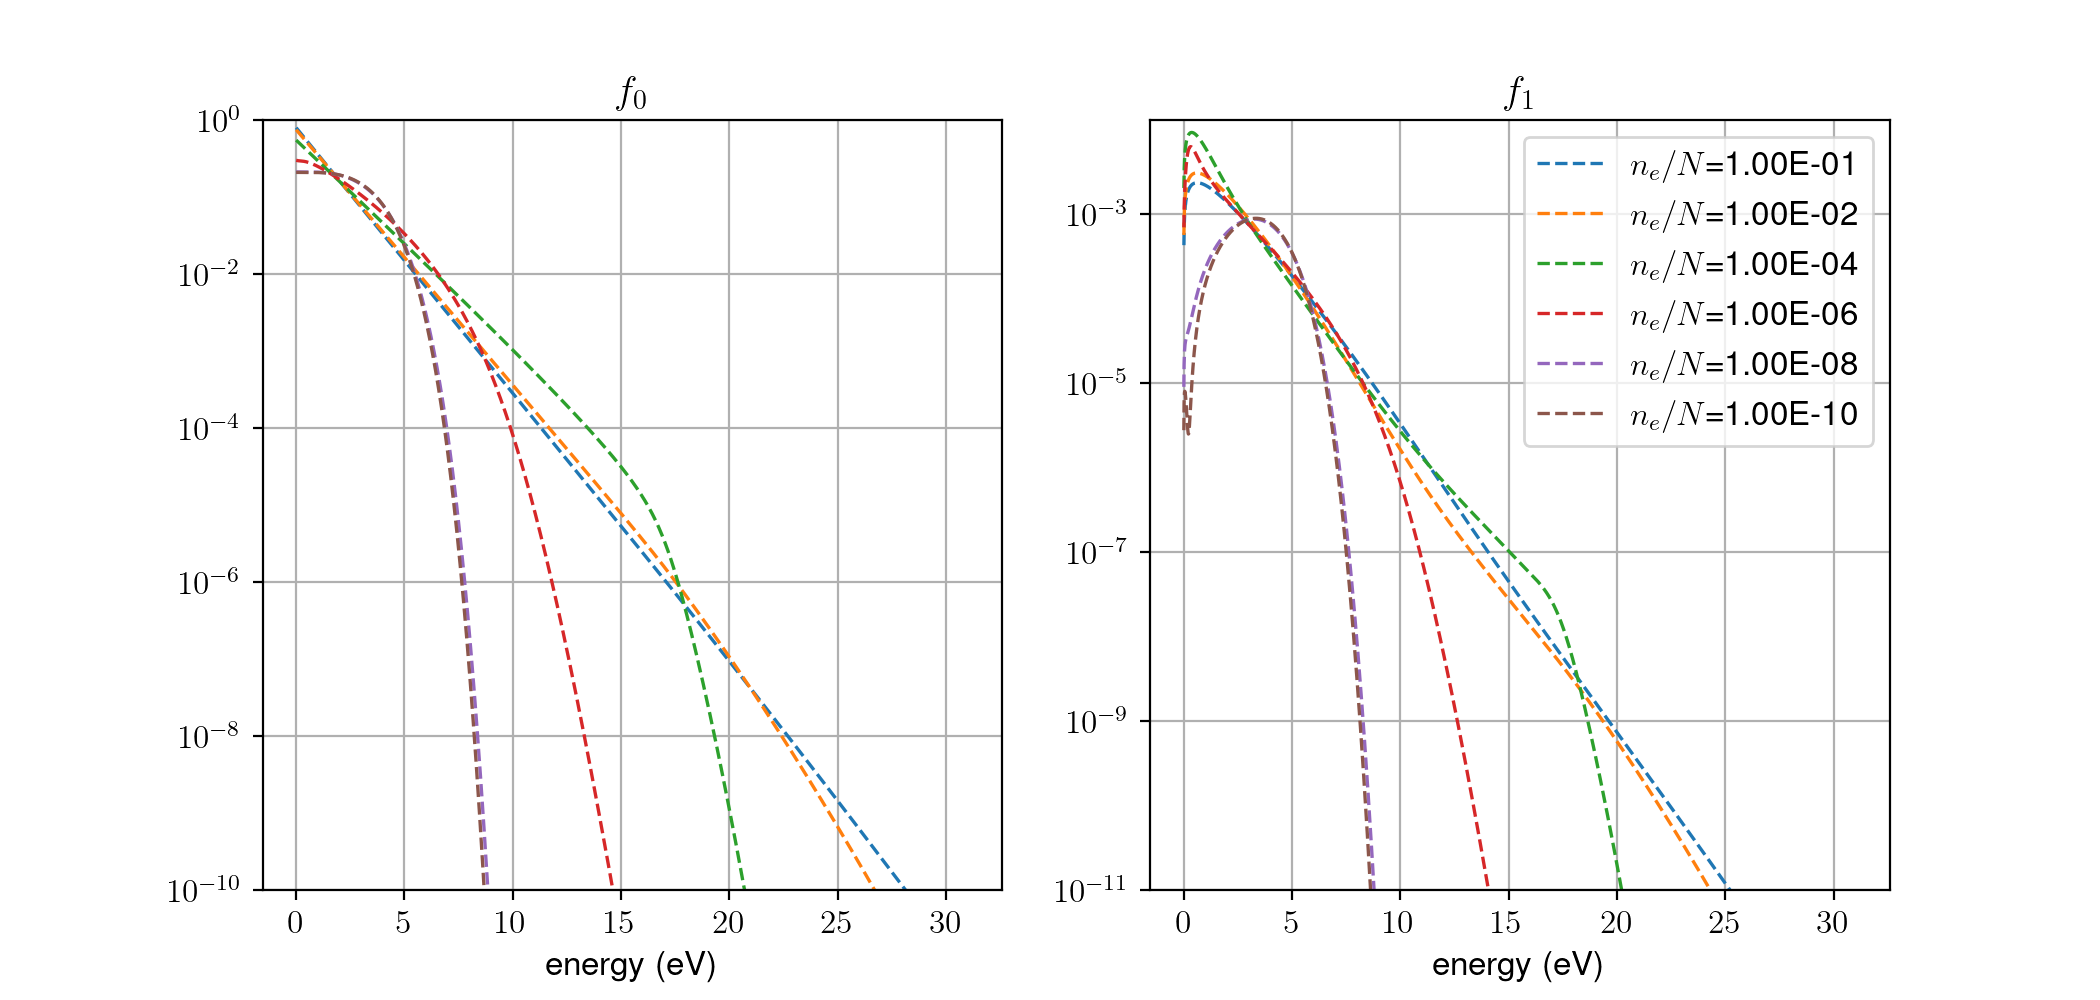
\includegraphics[width=0.85\textwidth]{1Td_cc.png}
	\end{center}
\end{frame}

\begin{frame}
	\frametitle{Boltzmann solver verification}
	\begin{itemize}
		\item We use Bolsig\footnote[frame]{Hagelaar, G.J.M. and Pitchford, L.C., 2005. Solving the Boltzmann equation to obtain electron transport coefficients and rate coefficients for fluid models. Plasma sources science and technology, 14(4), p.722.} code for verification step 
		\item Bolsig+ fixed two term approximation $f(\vect{v},t) = f_0(v, t) + f_1(v,t)\cos v_\theta$, assumes higher order correction terms negligible
		\item finite differences with uniform grid in energy
		\item supports steady state solutions or time-harmonic 
	\end{itemize}
\end{frame}

\begin{frame}[fragile]
	\frametitle{Verification with Bolsig+ code}	
	\begin{center}
		\only<+>{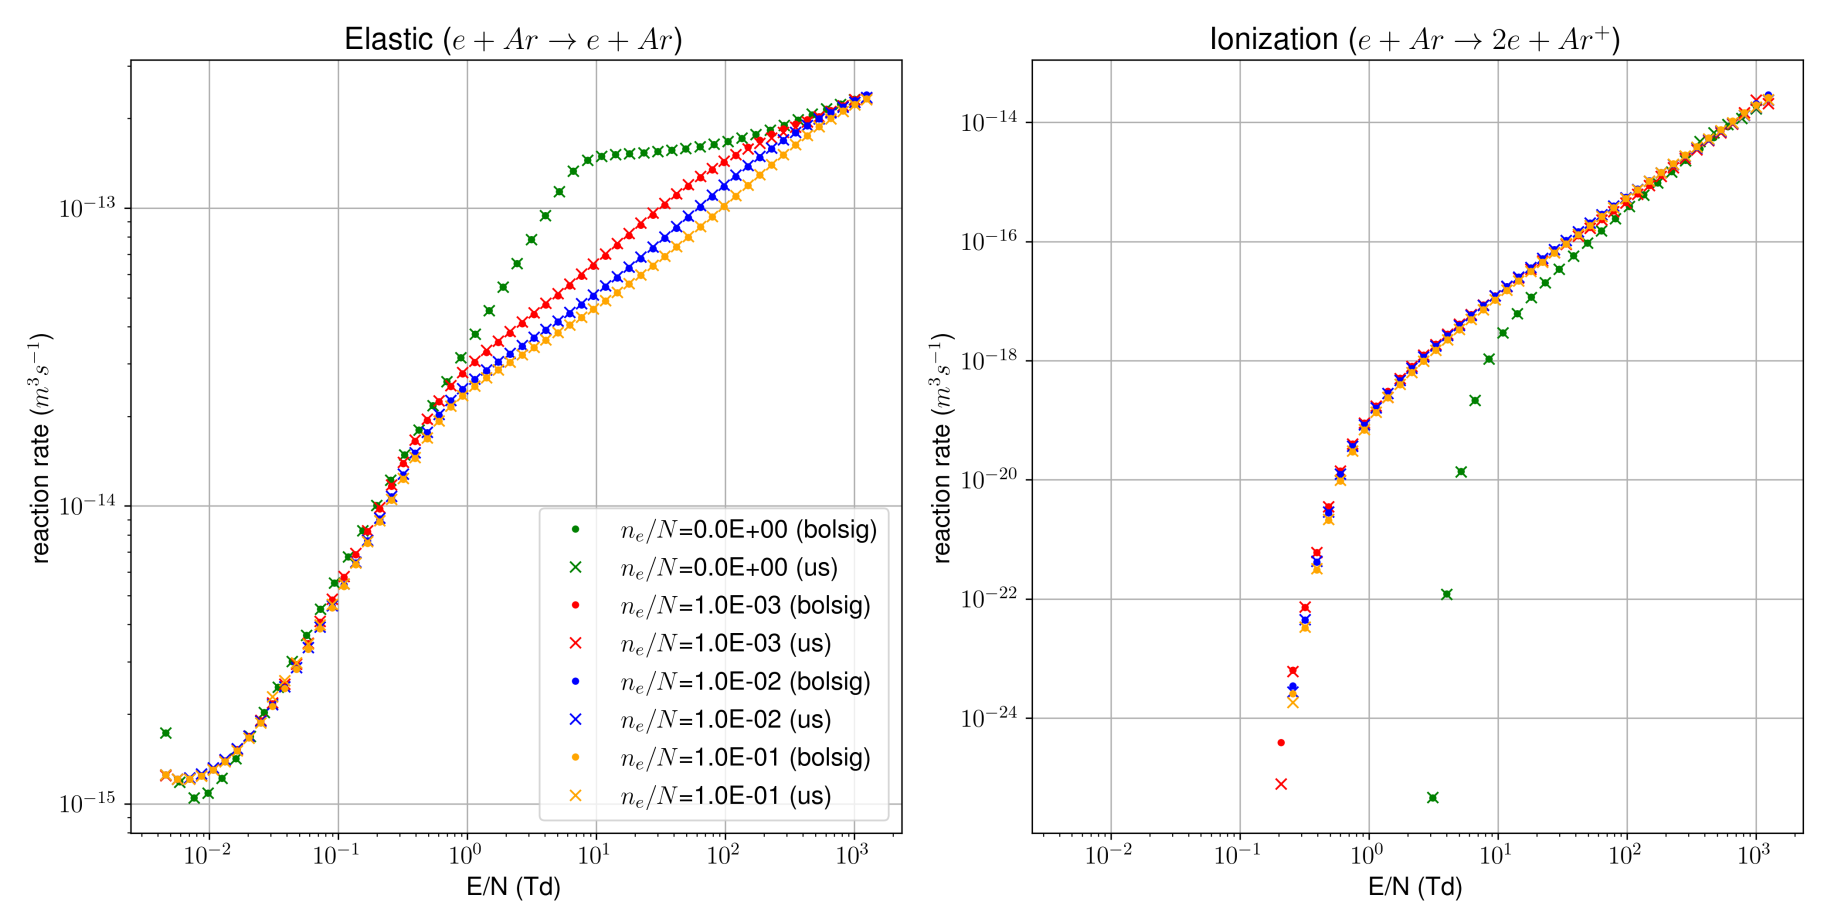
\includegraphics[width=0.9\textwidth]{pde_vs_bolsig_with_coulomb_collision1.png}}
		\only<+>{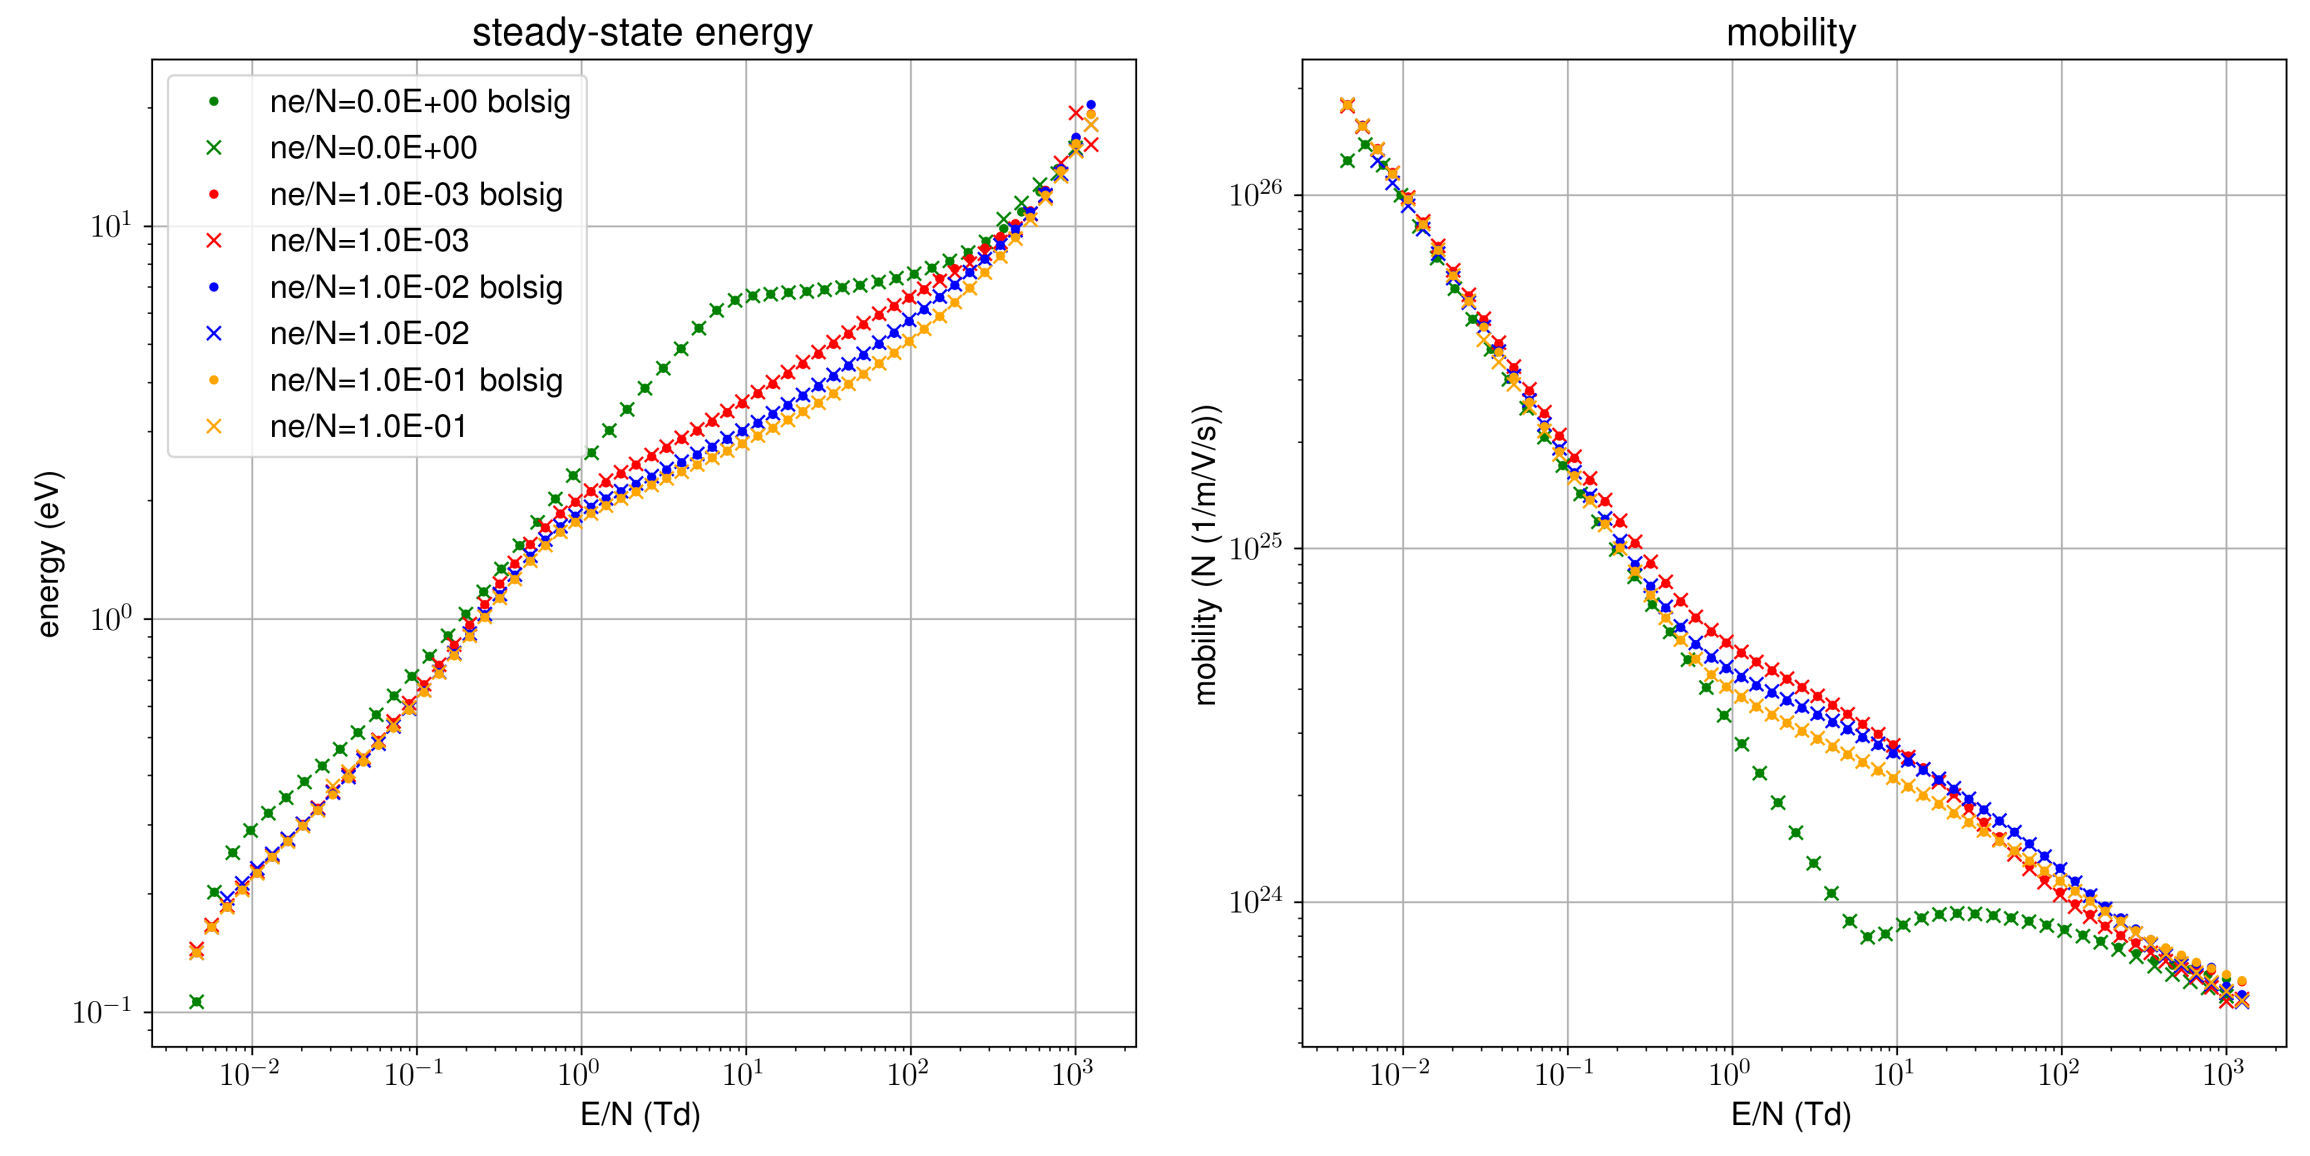
\includegraphics[width=0.9\textwidth]{pde_vs_bolsig_with_coulomb_collision2.png}}
	\end{center}
\end{frame}

\begin{frame}[fragile]
	\frametitle{Verification with Bolsig+ code}
	\vspace{-0.1in}
	\begin{center}
		\resizebox*{0.63\textwidth}{!}{
		\renewcommand{\arraystretch}{1.2}
		\begin{tabular}{|p{1cm}|p{1cm}|c|c|c|c|c|c|}
			\hline
			\multirow{2}{1cm}{\textbf{E/N (Td)}} & \multirow{2}{1cm}{\boldmath$n_e/N$} & \multicolumn{3}{c|}{\textbf{rel. error vs. Bolsig}} & \multicolumn{3}{c|}{\textbf{rel. error (self convergence)}}\\
			% \hline
			% \textbf{Inactive Modes} & \textbf{Description}\\
			\cline{3-8}
			& & \textbf{elastic} & \textbf{ionization} & \textbf{mobility} & \textbf{elastic} & \textbf{ionization} & \textbf{mobility}\\
			%\hhline{~--}
			\hline
			1        & 0.0 & 7.11E-05 &    --	    & 4.10E-05	& 4.61E-12	&   --	    & 2.47E-12 \\
			5        & 0.0 & 4.12E-04 & 3.74E-04	& 2.92E-06	& 3.83E-07	& 3.84E-04	& 5.34E-07 \\
			20       & 0.0 & 5.76E-04 & 3.49E-03	& 2.98E-04	& 2.77E-04	& 9.74E-03	& 1.29E-03 \\
			100      & 0.0 & 1.35E-03 & 2.74E-03	& 4.85E-03	& 2.02E-03	& 4.11E-02	& 6.65E-04 \\
			\hline
			1        & $10^{-3}$ & 9.40E-03	& 4.40E-03	& 7.99E-03	& 8.61E-07	& 3.60E-05	& 6.40E-07 \\
			5        & $10^{-3}$ & 1.52E-02	& 4.12E-03	& 1.83E-04	& 1.66E-07	& 1.42E-06	& 1.31E-07 \\
			20       & $10^{-3}$ & 1.69E-02	& 1.46E-02	& 1.13E-02	& 6.93E-08	& 1.89E-07	& 6.68E-08 \\
			100      & $10^{-3}$ & 9.11E-03	& 1.87E-02	& 1.65E-02	& 1.53E-07	& 2.96E-07	& 2.50E-07 \\
			\hline
			1        & $10^{-2}$ & 4.88E-03	& 1.20E-02	& 9.94E-03	& 6.72E-06	& 1.77E-04	& 5.18E-06 \\
			5        & $10^{-2}$ & 7.85E-03	& 8.73E-03	& 9.56E-03	& 2.73E-07	& 4.87E-06	& 2.07E-07 \\
			20       & $10^{-2}$ & 1.13E-02	& 4.57E-03	& 6.19E-03	& 1.85E-08	& 4.32E-08	& 1.48E-08 \\
			100      & $10^{-2}$ & 1.19E-02	& 9.93E-03	& 7.76E-03	& 2.50E-08	& 3.24E-09	& 2.57E-08 \\
			\hline
			1        & $10^{-1}$ & 1.72E-03	& 8.17E-03	& 5.31E-03	& 4.39E-05	& 6.37E-04	& 4.01E-05 \\
			5        & $10^{-1}$ & 2.42E-03	& 7.80E-03	& 7.74E-03	& 5.49E-06	& 5.91E-05	& 4.79E-06 \\
			20       & $10^{-1}$ & 3.84E-03	& 7.97E-03	& 8.41E-03	& 5.46E-07	& 5.01E-06	& 4.59E-07 \\
			100      & $10^{-1}$ & 4.76E-03	& 9.80E-04	& 1.89E-03	& 3.97E-08	& 2.88E-07	& 3.35E-08 \\
			\hline
		\end{tabular}}
		%\caption{Deterministic approach self convergence and comparison with the Bolsig code}
	\end{center}
\end{frame}



\begin{frame}
	\frametitle{Beyond two-term approximation}
	$E/N$ = 20Td, $n_e/N$=1e-2 with elastic + ionization + columbic collisions
	\begin{center}
		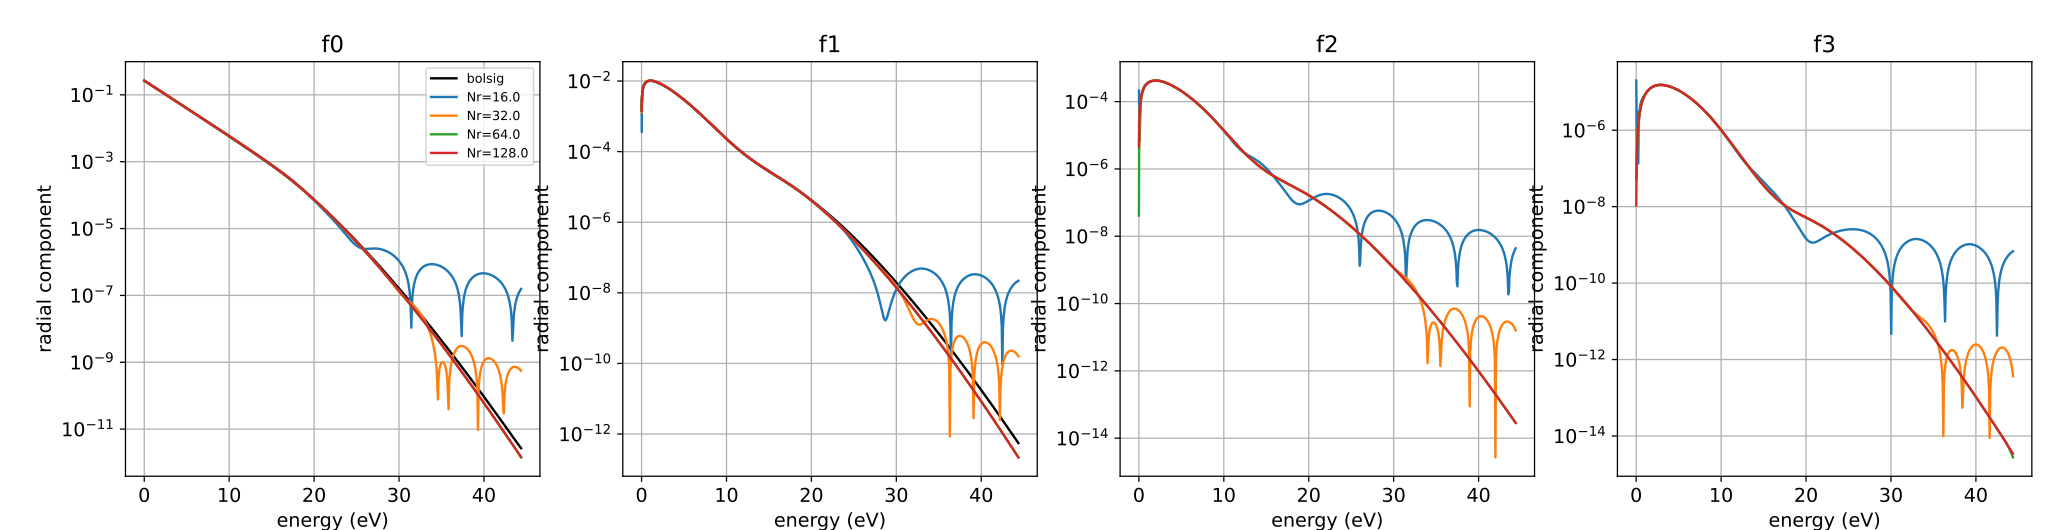
\includegraphics[width=\textwidth]{20Td_lmax3_ion_deg_1e-2.png}
	\end{center}
	\begin{itemize}
		\item Higher order modes triggered by larger E field and/or boundary conditions
		%\item Stronger $E$ field $\rightarrow$ trigger anisotropy, can makes the higher order modes significant to ignore.
		%\item Specially close to the boundaries of the torch application
	\end{itemize}  
\end{frame}

\begin{frame}
	\frametitle{Beyond two-term approximation}
	$E/N$ = 5Td, $n_e/N$=1e-3 with elastic + ionization + columbic collisions, T=3e-8 s
	\begin{center}
		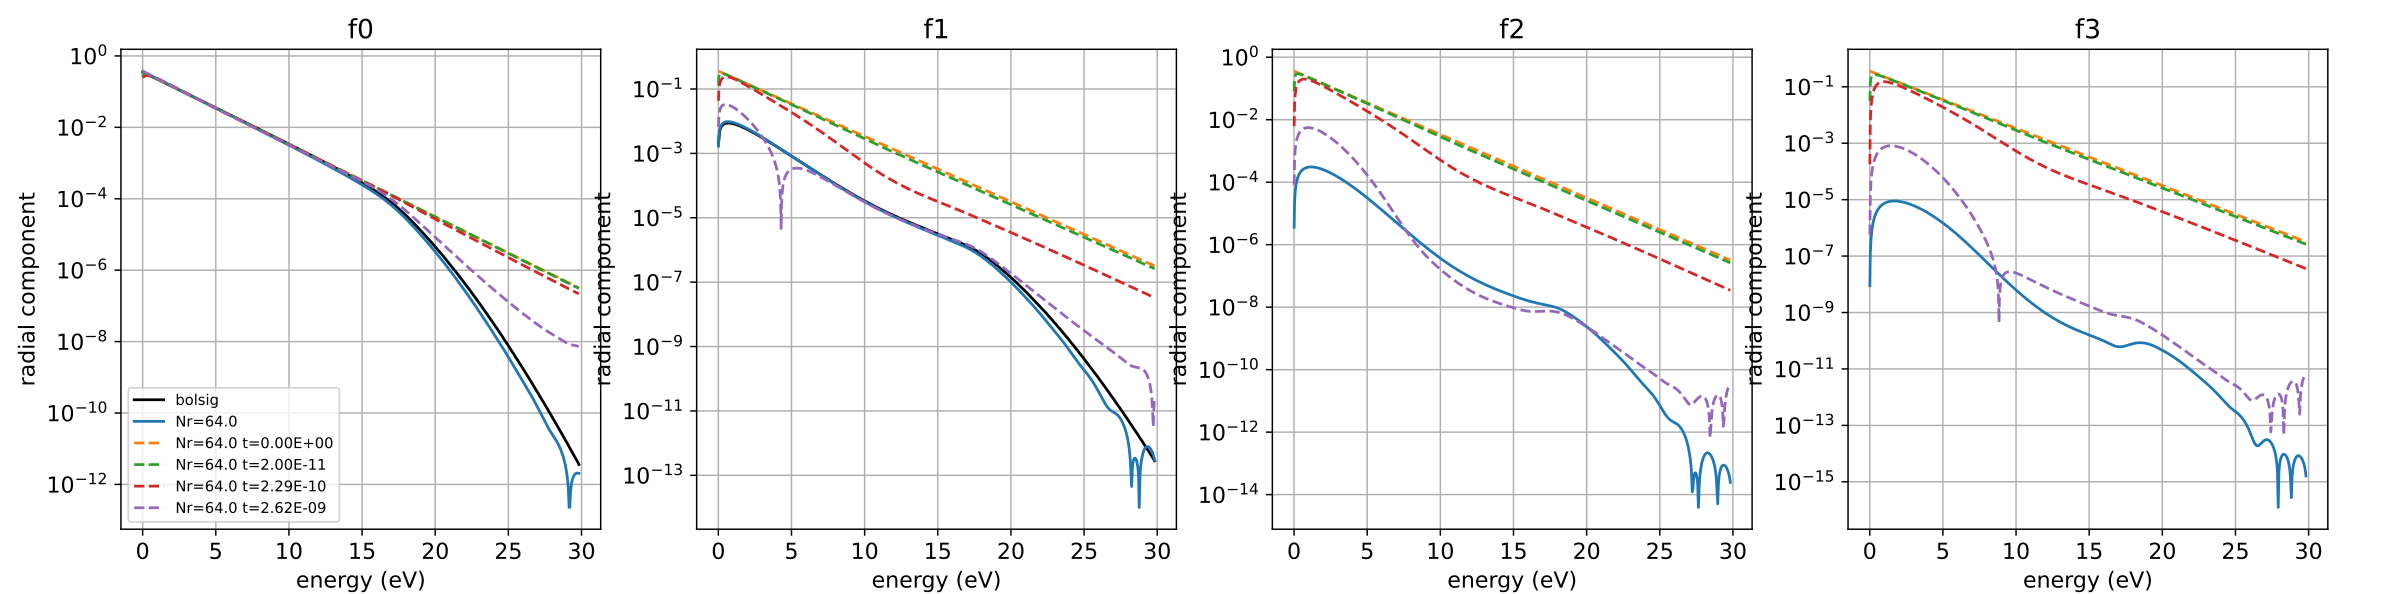
\includegraphics[width=\textwidth]{5Td_transient_ion_deg_1e-3.png}
	\end{center}
	\begin{itemize}
		\item Relaxation time $\tau$ for the higher order modes, if $\tau > \tau_{torch}$ $\Rightarrow$ higher order terms maybe significant
	\end{itemize}
\end{frame}

\begin{frame}
	\frametitle{Conclusions}
	\begin{itemize}
		\item B-Splines + spherical harmonic based continuous Galerkin formulation for v-space Boltzmann eq.
		\item Linear in $f$ collision terms (i.e., elastic, ionization, excitation)
		\item Support for electron-electron collisions with symbolic code generation
		\item \textbf{Beyond two-term expansion}: Generalization to higher order correction terms 
		\item Open-source Python based implementation
		\item Ongoing work
		\begin{itemize}
			\item Integration with PyKokos and Parla + HPC 
			\item Initial 1D + 3V approximation for the torch application
		\end{itemize}
		%\item Artificial diffusion in speed, for stabilization ?
	\end{itemize}
\end{frame}

\begin{frame}
	\centering
	\Huge Questions ? \\
	\centering
	\Huge Thank You. 
\end{frame}


\end{document}
